\chapter{Simulation Optimisation with Aspect Orientation}\label{chap:exp1_simulation_optimisation}

With a game deployed to experiment participants and a dataset of empirical play
collected, it was possible to determine optimal play in any game state. This
entirely separate body of work is documented in another student's PhD
thesis\inline{Cite William's PhD thesis}. This dataset leads to
further research. If we understand how players \emph{should} play, and we have
data to indicate how they \emph{do} play, we can investigate how real-world
players might be modelled. 

\section{Aims}\label{sec:aop_simulation_optimisation_aims}

Aspect orientation's use in previous simulation and modelling efforts have
typically focused on the use of aspects to compose model or simulation
details\inline{There must be tons of good citations for aspects being used to
compose together a simulation / model}. Critics of aspect orientation note that
the act of process composition makes visually understanding codebases difficult,
and so ensuring that a simulation properly models real-world behaviour is made
trickier with the introduction of aspect orientation. However, aspect
orientation might instead be used to \emph{augment} an existing model, by
rethinking what aspects are used to represent.

An alternative use of aspects would be to first build a non-aspect-oriented
model of \emph{expected} behaviour, and separately build aspects which describe
deviations from this. For example, one might more realistically simulate safety
procedures by first producing an idealised, ``naive'' model of what employees
are expected to do, and separately model alterations to prescribed behaviour as
an employee's boredom, expectation that checks and balances are unneccesary
wastes of their time, and so on --- effectively, separating out models of
degraded modes\cite{johnson2007degradedmodes}.

Previous research on the use of aspect orientation to model degraded modes
adopted the traditionally claimed benefit of aspect orientation: separation of
cross-cutting concerns, allowing for a greater reusability of
codebases\cite{wallis2018caise}. A repository of cross-cutting concerns in
socio-technical simulation such as boredom was developed as a library to be
applied to any future models\cite{fuzzimoss_repo}. However, aspects used in
simulation have no intrinsic need to represent concerns that are cross-cutting.
Indeed, whether they can be accurately used to represent cross-cutting concerns
in simulation is the topic addressed in \inline{Add a cross-reference to the
chapter on cross-cutting concern simulation accuracy when it exists}. Aspects
might instead be used to represent \emph{amendments to processes} which deviate
from an expected norm, in this case represented by the idealised model aspects
are applied to.

To more concretely relate this to the experiment at hand: play of RPGLite can be
modelled as players matchmaking, picking characters, and then mutually taking
turns until one player's characters are entirely expired. Once a player's
characters are dead, new matches can be made. This can continue indefinitely.
Lacking a heuristic to select next moves or characters, players might be
modelled as picking random moves. However, heuristics for move selection can be
added to the naive model of play by way of augmenting the processes already
defined through aspects. This approach can be of significant utility in both
modelling player behaviour and accurately modelling different players:

\begin{enumerate}
    \item Different players might use their own unique heuristics to model play.
    Each player's behaviour is therefore well described by separating what play
    ``looks like'' to what makes a given player play differently to their peers.
    \item Different players might lean more heavily on different heuristics, or
    mixes thereof. Play might be characterised by reliance on experience, on
    recent games, on knowledge of an opponent, and so on; these different
    variables can be expected to be weighted differently by each player, adding
    complexity to the code which models this individualised play.
    \item A modeller might discover a new idea for a heuristic long after
    developing an original concept for a model. The easiest methods for amending
    the original model should require the least rewriting of original code. Due
    to the impact of \pointno{2}, ideal architectures for an approach such as
    this should require these heuristics to be defined entirely separately to
    the base model.
\end{enumerate}

Considering \pointno{1}, \pointno{2}, and \pointno{3}, architectures and
paradigms which enable separation of concerns are well-suited to defining
alternative approaches to play. Some architectural approaches such as mixins or
plugin design patterns might support this structure well, but they typically
rely on language features (in the case of mixins) or knowledge of software
engineering (in the case of design patterns). Aspect orientation is typically
provided to developers as a framework or runtime in a language (such as
AspectJ\cite{aspectj_intro} or PROSE\cite{popovici2002PROSE}) and can require
minimal architectural understanding to use: concepts are simple, and the effort
of composition is alleviated by the supporting framework or runtime.

The approach makes little use of aspect orientation's significant contribution
--- cross-cutting concerns --- as whether behaviour cross-cuts different parts
of a codebase is not of interest in this use case. Instead, aspect orientation
is treated as a composition mechanism with a reasonably low degree of technical
knowledge required.

\subsection{PyDySoFu Suitability}\label{subsec:optimisation_with_aspects_usingpdsf}
Some aspect orientation frameworks do not adequately achieve this requirement.
For example, the most influential framework, AspectJ, requires the use of
language extensions to define integrate aspect
orientation\cite{AspectJLanguageAndTools}, and similar additional complexity is
added in seemingly every alternative framework, through the use of bespoke
virtual machines, compilers, translators, or
languages\cite{rajan2006nu_towardsAO_invocation,popovici2003JITaspects,AspectCplusplusDesignImpl,baker2002maya}.

PyDySoFu, however, requires very little additional knowledge to use. Its design
prioritises simplicity and a shallow learning curve that makes its adoption by
researchers without a software engineering background feasible: \inline{maybe
cut this list of reasons PyDySoFu is fantastic...}

\begin{itemize}
    \item PyDySoFu is implemented as a pure-python library, meaning that it can
    be installed through Python's package manager (pip) and imported like any
    other Python library. No additional supporting infrastructure is required.
    \item Aspects in PyDySoFu are simple functions which take as arguments
    whichever pieces of information are pertinent for the function's use as an
    aspect\footnote{For example, an ``encore'' aspect which is woven after a
    target procedure returns will be provided that target's return value.}.
    \item To weave a PyDySoFu aspect requires only a method call, which returns a
    \lstinline{callable} which unweaves that aspect.
    \item Defining PyDySoFu pointcuts requires only a regular expression
    matching a method name. This can apply to a wide range of join points if
    required, but where method names are provided directly, the join point is
    made clear.
    \item Additional clarity over where aspects \emph{can} be woven is
    introduced by PyDySoFu's transparent weaving of aspect hooks, mitigating
    some of aspect orientation's most prominent criticisms.
\end{itemize}

PyDySoFu therefore satisfies the requirements of this work well: it offers
composition of procedures outside of the scope of an original codebase, makes
what is being composed where clear to a programmer, and makes no significant
changes to Python as a language (thereby requiring users to specialise in fewer
tools). 


\subsection{Proposed Experiment}\label{subsec:optimisation_with_aspects_experiment}

Aspect orientation's use as a composition tool for model components makes sense
in principle, but it is unclear whether the addition of behaviours to a naive
model would make the model more ``realistic''. Furthermore, changes to a model
could alter its representation so as to weaken its mimicry of the system it
simulates; adding behaviours could make it \emph{less} realistic. The
fundamental issue at play is that it is unclear whether the changes made would
properly represent what might be empirically observed. While PyDySoFu's design
makes understanding what is being composed simpler than other aspect orientation
frameworks, a composed model under this paradigm is still split across multiple
areas of a codebase, making a visual assessment of whether a model accurately
reflects the intended behaviour impractical. It is therefore important to
demonstrate the efficacy of PyDySoFu and the modelling paradigm it introduces,
by confirming the realism of a model to which behavioural variation is applied.

We can confirm whether aspects can realistically represent changes to a naive
understanding of the real world by comparing their output against empirical
data. For example, if a such a model of behaviour in a system outputs data which
correlates poorly against empirically collected data, a change to that system
would make it more realistic if it improved this correlation, and could be said
to be realistic if the generated data appeared sufficiently ``close'' to the
empirical dataset --- which here means that the correlation between the two is
of statistical significance. Such a change can be aspect-oriented. Therefore, we
can see the application of aspects as the application of packages of potential
improvements to a base model, which can be verified by way of comparison to
known-good datasets.

This is the basis of the experiments in this thesis.

With datasets collected empirically on RPGLite's play, we can build a naive
model of play and aspects to apply that should realistically model data from
players. This can be used to answer the question:

\begin{researchquestion}
    Can aspect-oriented models be said to exhibit realism?
\end{researchquestion}

% To answer this question, a naive model of play is produced, and aspects
% developed which encapsulate different play styles so as to compare empirically
% sourced datasets against both its aspect-augmented and unaltered counterparts.
% The following subsections detail the naive model developed and aspects applied
% to this model.

To answer this question, a naive model of play is produced. Aspects are
developed which model learning within the system defined by the naive system.
The synthetic datasets produced by models with naive or aspect-applied models
can be compared to an empirical dataset sourced from real-world players of the
game, and their similarity compared. 

``Naive'' is used here to describe a model which does not encode any
understanding of the players of the game being modelled. Traits such as
learning, distraction, or aptitude for similar games are irrelevant to the naive
model. We need a naive model to demonstrate the effectiveness of an
aspect-oriented alternative: we can measure how closely it reflects empirical
data, and compare this against the same measurement drawn from another model
with behavioural variations encoded using aspects. A closer match from our
aspect-oriented model would demonstrate that the technique can enhance a model's
realism. Our naive model also provides a null hypothesis: if no improved
similarity is observed, the technique brought no improvement to the model's
realism. No measurable difference indicates that weaving behavioural variations
as aspects has no impact on a model's realism.

\inline{Write a little here on the learning aspects.}

\inline{Flesh this out as a brief wrap-up of our experimental technique. The end
of our ``naive'' model explanation might be useful to move down here / rework
into this para.} Contrasting the similarity of the empirical dataset to both
naive and aspect-applied datasets\ldots{} This discussion is provided so as to
provide context for the following sections; experimental design is discussed in
more depth in \cref{sec:optimisation_with_aspects_experimental_design}. 


\section{Naive Model}\label{sec:optimisation_with_aspects_naivemodel}

A naive model of play was developed by separating each stage of the actions
taken by players in the client-side app, and separating them into individual
procedures. 

To facilitate the retrieval of information pertinent to a simulation in an
applied aspect, the model was written so as to contain simulation state as
mutable function arguments. The model was written as a workflow, and state of
workflow execution was separated into three components: the actor that a
function invocation (or ``step'') represents activity from; the context of that
step in the execution of a workflow; and the context of that workflow's
execution in a broader environment. Incidentally, we found this structure to
allow a flexible and natural implementation of a procedural simulation, which
should translate easily to existing simulation frameworks such as
SimPy\cite{simpy_intro}:

\begin{description}
  \item[Actor ---] allows the function to identify the actor performing the activity
    defined by the function. This argument is any object uniquely identifying an
    actor.
  \item[Context ---] allows the function to determine details of the current
    thread of work being undertaken by the actor. This is necessary because in
    some simulations, the same actor might pause and resume multiple occurrences
    of the same activity --- for example, they might concurrently play three
    different matches in RPGLite. As a result, it is necessary to understand the
    context of the action being performed by the actor in question. This
    argument can be any object uniquely identifying the context of a piece of
    work, but should be mutable (such as a class or dictionary-like object) to
    permit the communication of information across invocations of different
    action-representing functions.
  \item[Environment ---] an actor's actions are often determined by the global
    environment they act within. There may be ancillary details to the
    actor's actions and the context of their particular thread of work which
    they are undertaken within which are used to determine behaviour, such
    as a landscape they traverse or other actors they might choose to
    interact with. Because all actors share access to a global environment,
    this also provides a message passing space, or a space where actors can
    set values and flags other actors might look to, should those details be
    more general than their specific thread of work at a given point in time.
    \footnote{This is different to environments in some other simulation frameworks, such
    as SimPy\cite{simpy_documentation}, where the environment controls scheduling and
    execution: this structure imposes no constraints such as models of time, and
    anticipates that any such functionality should be implemented by the
    programmer. However, an environment such as SimPy's might satisfy a programmer's needs
    when using this particular pattern.}
\end{description}

Each simulation step receives these three arguments at a minimum. Because steps
of the model are functions, and therefore valid join points, aspects applied to
these have access to the entire state of the simulation.

The naive model of RPGLite follows a simple workflow mimicking player
interaction with the client-side application used by real-world players.
A graphical representation is provided in \cref{fig:naive_model}. \inline{Position this figure properly on the page.}
\inline{Maybe reword? Pretty verbose.} The model it describes produces synthetic data.
It does so by simulating players interacting with each other in a broader
RPGLite ecosystem. The large number of players is important: future behavioural
variations introduce behaviours which guide future actions based on past
experiences. Non-determinism early in the model can therefore cause different
players to act in different ways. Simulating many players allows the system to
represent a wide variety of early experiences, as would occur to real-world
players, too. As the aspects being woven simulate learning, early experiences
which cause players to learn maladaptive strategies --- or simply strategies
less optimal than those learned by their peers --- should later contrast against
winning strategies, so that players with less useful early inferences can learn
from players who play more optimally.

\begin{figure}
  \centering
  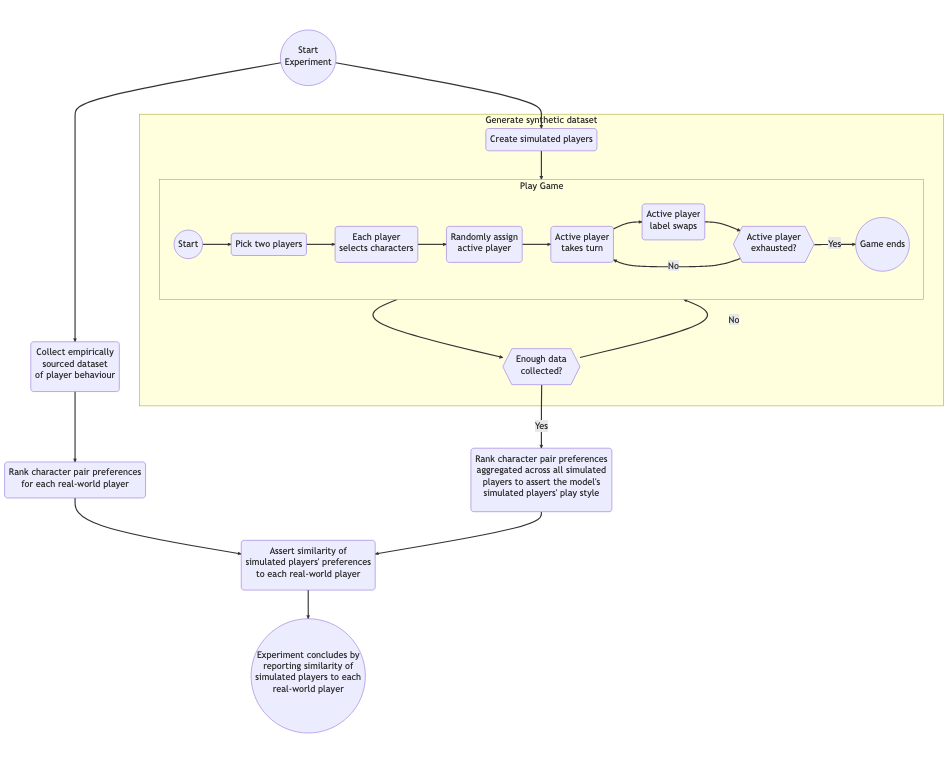
\includegraphics[width=\columnwidth]{50_optimisation_with_aspects/diagrams/naive_model.png}
  \caption{A flowchart diagramming a simple model of RPGLite play, without
  aspects applied.}
  \label{fig:naive_model}
\end{figure}


\inline{Consider changing \cref{fig:naive_model} to only include details about
the model of the game itself, leaving the steps about data analysis to the
later aspect-applied version (which is the real experiment).}
\inline{Move \cref{fig:naive_model} to .svg for fidelity}
The stages of the naive model as laid out map to those encountered by real-world
players. Two randomly-selected players repeatedly select characters to play
(from the pool of 8 characters available in the real-world game), and a player
is chosen to play first at random. That player selects a random valid move to
make.\footnote{Many simulated decisions are random; this is because the model is
designed to be naive, so it avoids informed decisions where possible. Informed
decisions are expected to be woven later as aspects.} The active player alternates, and the process repeats, until
such time as an active player starts their turn with both of their characters
fully depleted of health. The player with remaining characters is the victor,
and another game is started by picking random players and starting a game
between them, until a predetermined number of games has been played.

After a sufficient number of games are played, analysis of the various datasets
collected can begin, although this is discussed in more detail in
\cref{sec:optimisation_with_aspects_experimental_design}.




\section{Experimental Design}\label{sec:optimisation_with_aspects_experimental_design}

Having discussed the aspects to apply above, this section describes how we'll
apply those aspects to compare simulations under variation to controlled
simulations, and how such an experiment answers our research question.

This likely won't need any subsections: we've already laid out the groundwork
above as to what's involved technically, so this is statistical, explanation of
our control, our model under test, and how they'll be compared in a rigorous and
scientifically appropriate manner.

However, this \emph{should} lay out the rationale behind simulating learning
with our aspects; we'll discuss how our datasets are compared here, and how we
measure similarity, which is done by proportion of classes picked over time.
There are statistical and methodological requirements at play here --- we needed
something we could compare in a statistically significant manner --- but also,
we needed something which the dataset we had could support analysis of. We only
had a few players with statistically significant numbers of games played.
Character choice seemed a reasonable way to go, because the metagame introduces
specific character combinations which are optimal, and we'd expect players to
learn those over time. Players \emph{might} get stuck in local minima, but
learning aspects would too, so simulated player data should still reflect that.
Also, the choice of an ideal team composition is a well-understood aspect of
metagame design \inline{Is team composition in metagame design something there's
also literature on, or is this only within the gaming industry?}, so we can
imagine players optimising team composition in RPGLite like they would in other
trading card or RPG games.


\section{Aspects Applied}\label{sec:optimisation_with_aspects_aspectsdeveloped}

% Players can be expected to select stronger characters as they understand
% gameplay more. Aspects were therefore developed to track player experience with
% characters. As players became more familiar with the characters they play, we
% can hypothesise that they will better understand how to play with those
% characters, and more often select characters they have success with. 

\inline{Write about \emph{both} aspects so as to answer the hypothesis : Can
aspects be used to generate models of alternative behaviours?}

The aim of this experiment is to investigate whether a model with
aspect-oriented behavioural variation can be realistic; the experiment therefore
requires the development of aspects representing plausibly realistic behavioural
variation. Traces from simulations affected by these aspects should produce
synthetic data which can be compared to real-world data and to naive data,
enabling the measurement of the datasets' similarity, as discussed
in~\cref{sec:optimisation_with_aspects_aspectsdeveloped}. 

To demonstrate that simulated players are plausibly realistic, and
that a simulation's realism can be improved by the addition of behavioural
variance as a cross-cutting concern, naive player behaviour is augmented by
applying aspects which represent learning. Two methods of learning RPGLite's
metagame were produced; this section will detail both.

In each model of learning, players are assumed to have a draw towards choosing
to play some characters, and less of a draw to others. This draw is informed by
whether players have reason to believe they'll be successful after choosing a
given character; players' future decisions are informed by the outcomes of their
previous ones. The models of leaning presented in this section are
differentiated by the manner in which future decisions are informed.

\inline{Why didn't we make a bayesian model of learning? Should we have? Would this be difficult at all?}

\subsection{Simple Model of Learning}\label{subsec:optimisation_with_aspects_basiclearningaspect}

\inline{Describe probability updates by way of a simple PMF defined by previous outcomes}




\subsection{Modelling Bias with Hyperbolic Decay}\label{subsec:optimisation_with_aspects_hyperbolicdecay}

\inline{Find citations explaining hyperbolic decay}

\inline{Describe probability updates affected by a hyperbolic decay bias}





\section{Experimental Results}\label{sec:optimisation_with_aspects_experimental_results}

Presentation of the results owing from the experiment as described in
\cref{sec:optimisation_with_aspects_experimental_design}, and evaluation of the
research question with respect to these findings.

Again, no subsec likely required here.

\section{Discussion}\label{sec:optimisation_with_aspects_discussion}

A closing discussion on what we found, and how the research question was
answered.